  % ============================================================
%  DoRA Multi-Modal Research Poster — Cornell Red Theme
%  36 x 24 inches  (91.44 x 60.96 cm)
%
%  Cornell logo: drop cornell.png in this folder.
%  If absent, the TikZ fallback seal is used automatically.
% ============================================================
\documentclass[final]{beamer}

\usepackage[size=custom,width=91.44,height=60.96,scale=1.2]{beamerposter}
\usepackage{amsmath,amssymb,bm}
\usepackage{booktabs}
\usepackage{tabularx}
\usepackage{graphicx}
\usepackage{xcolor}
\usepackage{tikz}
\usepackage{pgfplots}
\pgfplotsset{compat=1.18}
\usepackage[most]{tcolorbox}
\usepackage{microtype}
\usepackage{ragged2e}
\usepackage{colortbl}
\usetikzlibrary{arrows.meta,positioning,shapes.geometric,calc}

% ----------------------------------------------------------
%  Cornell Palette
% ----------------------------------------------------------
\definecolor{CornellRed}   {RGB}{179, 27,  27}
\definecolor{CornellDark}  {RGB}{ 91,  0,   0}
\definecolor{CornellMid}   {RGB}{140, 20,  20}
\definecolor{CornellAccent}{RGB}{220,170,170}
\definecolor{CornellLight} {RGB}{250,238,238}
\definecolor{CornellGray}  {RGB}{ 84, 88,  90}
\definecolor{LoRABlue}     {RGB}{ 60,100,165}
\definecolor{NumGreen}     {RGB}{ 30,120, 60}
\definecolor{BodyBg}       {RGB}{255,255,255}
\definecolor{TableShade}   {RGB}{253,238,238}

% ----------------------------------------------------------
%  Beamer base
% ----------------------------------------------------------
\setbeamercolor{background canvas}{bg=white}
\setbeamercolor{footline}{bg=CornellDark,fg=white}
\setbeamertemplate{navigation symbols}{}

% ----------------------------------------------------------
%  TikZ Cornell Seal (fallback)
% ----------------------------------------------------------
\newcommand{\CornellSealTikZ}[1][2.8cm]{%
  \begin{tikzpicture}
    \fill[CornellDark] (0,0) circle (#1);
    \fill[white]       (0,0) circle ({#1*0.84});
    \fill[CornellMid]  (0,0) circle ({#1*0.70});
    \fill[white]
      ({-#1*0.28},{#1*0.22}) -- ({-#1*0.28},{-#1*0.06})
      .. controls ({-#1*0.28},{-#1*0.32}) and (0,{-#1*0.44}) ..
      (0,{-#1*0.44})
      .. controls (0,{-#1*0.44}) and ({#1*0.28},{-#1*0.32}) ..
      ({#1*0.28},{-#1*0.06})
      -- ({#1*0.28},{#1*0.22}) -- cycle;
    \fill[CornellDark!80]
      ({-#1*0.28},{#1*0.22}) rectangle ({#1*0.28},{#1*0.10});
    \node[text=white,font=\fontsize{5}{5}\selectfont\bfseries]
      at (0,{#1*0.77}) {CORNELL UNIVERSITY};
    \node[text=white,font=\fontsize{4.5}{4.5}\selectfont]
      at (0,{-#1*0.77}) {FOUNDED A.D. 1865};
  \end{tikzpicture}%
}

\newcommand{\CornellLogo}[1][3.0cm]{%
  \IfFileExists{cornell.png}{%
    
\includegraphics[height=#1]{cornell.png}%
  }{%
    \CornellSealTikZ[#1]%
  }%
}

% ----------------------------------------------------------
%  Headline (6.5 cm — slim bar for more content space)
% ----------------------------------------------------------
\setbeamertemplate{headline}{%
  \begin{beamercolorbox}[wd=\paperwidth]{headline}%
    \begin{tikzpicture}
      \fill[CornellRed]  (0,0) rectangle (\paperwidth, 6.2cm);
      \fill[CornellDark] (0,0) rectangle (\paperwidth, 0.25cm);
      \node at (4.0cm, 3.4cm) {\CornellLogo[5.0cm]};
      \node[text=white,
            font=\fontsize{40}{46}\selectfont\bfseries,
            text width=78cm, align=center]
        at ({0.5*\paperwidth}, 4.5cm)
        {Exploring DoRA: Weight-Decomposed Low-Rank Adaptation Across Modalities};
      \node[text=white!92,
            font=\fontsize{24}{24}\selectfont, align=center]
        at ({0.5*\paperwidth}, 3cm)
        {Richie Xue \quad\textbullet\quad
         Shaurya Sen \quad\textbullet\quad
         Kyle Du};
               % Affiliation row
      \node[text=white, font=\normalsize]
        at ({0.5*\paperwidth}, 1.5cm)
        {Cornell University $\cdot$ Dept.\ of Computer Science
         $\cdot$ CS\,4782: Introduction to Deep Learning
         $\cdot$ Spring 2025};
      % \node[text=white!70,
      %       font=\fontsize{15}{18}\selectfont, align=center]
      %   at ({0.5*\paperwidth}, 1.2cm)
      %   {Cornell University \quad\textbullet\quad
      %    CS\,4782: Introduction to Deep Learning \quad\textbullet\quad
      %    Spring 2025};
    \end{tikzpicture}%
  \end{beamercolorbox}%
}

% ----------------------------------------------------------
%  Footline
% ----------------------------------------------------------
\setbeamertemplate{footline}{%
  \begin{beamercolorbox}[wd=\paperwidth,ht=1cm,dp=0.3cm]{footline}%
    \begin{tikzpicture}
      \fill[CornellDark] (0,1cm) rectangle (\paperwidth, 2cm);
      % References row
      \node[text=white!75, font=\fontsize{14}{17}\selectfont,
            text width=89cm, align=left, anchor=west]
        at (1.2cm, 1cm)
        {[1] Liu et al.\ (2024). DoRA. \textit{ICML}.\quad
         [2] Hu et al.\ (2022). LoRA. \textit{ICLR}.\quad
         [3] Wang et al.\ (2018). GLUE. \textit{EMNLP}.\quad
         [4] Warden (2018). Speech Commands. \textit{arXiv}.\quad
         [5] Kim et al.\ (2024). OpenVLA. \textit{arXiv}.\quad
         [6] Jiang et al.\ (2023). SmolVLM. \textit{HuggingFace}.\quad
         [7] Nasiri \& Garraghan (2025). EDoRA: Efficient Weight-Decomposed Low-Rank Adaptation via SVD. \textit{arXiv}:2501.12067.};
    \end{tikzpicture}%
  \end{beamercolorbox}%
}

% ----------------------------------------------------------
%  tcolorbox style
% ----------------------------------------------------------
\tcbset{
  posterblock/.style={
    enhanced,
    colback        = BodyBg,
    colframe       = CornellDark,
    colbacktitle   = CornellMid,
    coltitle       = white,
    fonttitle      = \large\bfseries,
    boxrule        = 0.5pt,
    arc            = 4pt,
    titlerule      = 0pt,
    top            = 0.30cm,
    bottom         = 0.30cm,
    left           = 0.40cm,
    right          = 0.40cm,
    toptitle       = 0.18cm,
    bottomtitle    = 0.18cm,
    before skip    = 0.40cm,
  },
  statbox/.style={
    enhanced,
    colback        = CornellLight,
    colframe       = CornellRed,
    boxrule        = 1pt,
    arc            = 4pt,
    top            = 0.20cm,
    bottom         = 0.20cm,
    left           = 0.20cm,
    right          = 0.20cm,
  }
}

\newcommand{\hl}[1]{\textcolor{CornellRed}{\textbf{#1}}}
\newcommand{\lb}[1]{\textbf{#1:}\;}
\renewcommand{\arraystretch}{1.2}

% Figure-or-placeholder helper: shows the image if present,
% otherwise a labelled grey box of the same width.
\newcommand{\FigOrBox}[3]{%
  % #1 = filename, #2 = width, #3 = placeholder caption
  \IfFileExists{#1}{%
    \includegraphics[width=#2]{#1}%
  }{%
    \fcolorbox{CornellAccent}{CornellLight}{%
      \begin{minipage}[c][0.55\linewidth][c]{#2}%
        \centering{\color{CornellGray}\small\itshape [Figure: #3]}%
      \end{minipage}%
    }%
  }%
}

% ----------------------------------------------------------
\begin{document}
\begin{frame}[t]
	\vspace{-1.5cm}

	\begin{columns}[T,totalwidth=\textwidth]
		\setlength{\columnsep}{0.8cm}

		% ============================================================
		%  COLUMN 1  —  Problem + Method + Setup  (v2)
		% ============================================================
		\begin{column}{0.31\textwidth}

			\begin{tcolorbox}[posterblock, title={The Problem}]
				Fine-tuning billion-parameter models is costly for most teams.

				\small\hl{LoRA} (Hu et al., 2022) helps by freezing the base weights $W_0$ and learning a low-rank update $BA$, but this update changes a layer's \emph{magnitude} (how strong) and \emph{direction} (what feature) \textbf{together}.

				\vspace{0.25cm}
				\small\hl{DoRA} (Liu et al., 2024) decouples them: learn magnitude as a separate scalar, and let LoRA update only the direction.
			\end{tcolorbox}


			\begin{tcolorbox}[posterblock, title={DoRA Architecture}]
				\begin{center}
					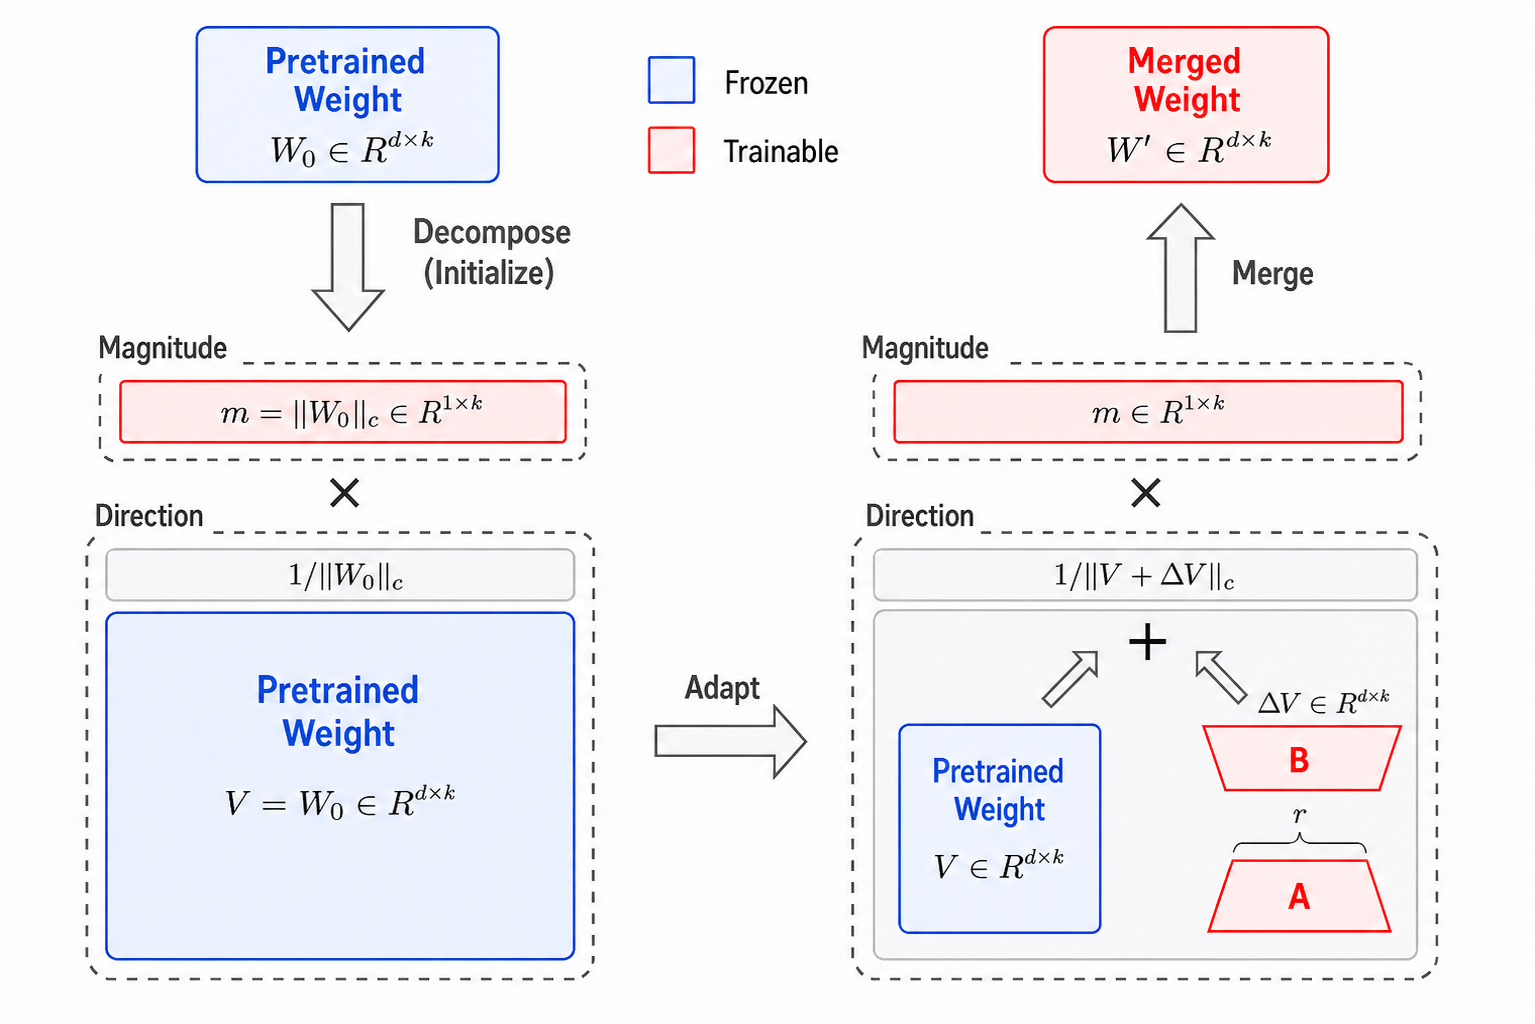
\includegraphics[width=0.7\linewidth]{dora_architecture.png}
				\end{center}
				\vspace{0.15cm}
				\small\textit{DoRA splits each weight $W_0$ into magnitude $m$ and direction $V/\lVert V\rVert_c$, applying a LoRA update $BA$ only to the direction while training $m$ as a separate scalar.}
			\end{tcolorbox}

			\begin{tcolorbox}[posterblock,title=Audio Results]
				Wav2Vec2-base (67M params) fine-tuned on Google Speech Commands
				v0.02 — 84.8k utterances, \textbf{12 keyword classes}.

				\vspace{0.2cm}
				\begin{center}\small
					\begin{tabular}{@{}lcccc@{}}
						\toprule
						\textbf{Method} & \textbf{Val Acc}   & \textbf{Test Acc}
						                & \textbf{Trainable} & \textbf{Time}      \\
						\midrule
						\rowcolor{TableShade}
						DoRA ($r=8$)    & \textbf{98.6\%}    & \textbf{89.7\%}
						                & 826.6k             & \textbf{183.6 min} \\
						LoRA ($r=8$)    & 98.5\%             & 89.0\%
						                & 789.8k             & 190.8 min          \\
						\bottomrule
					\end{tabular}
				\end{center}

				\vspace{0.15cm}
				\small\textit{\hl{+0.7\% test accuracy}.
					The magnitude scalar's small overhead is offset by faster directional
					gradient convergence on the audio encoder.}

				\vspace{0.25cm}
				\begin{center}
					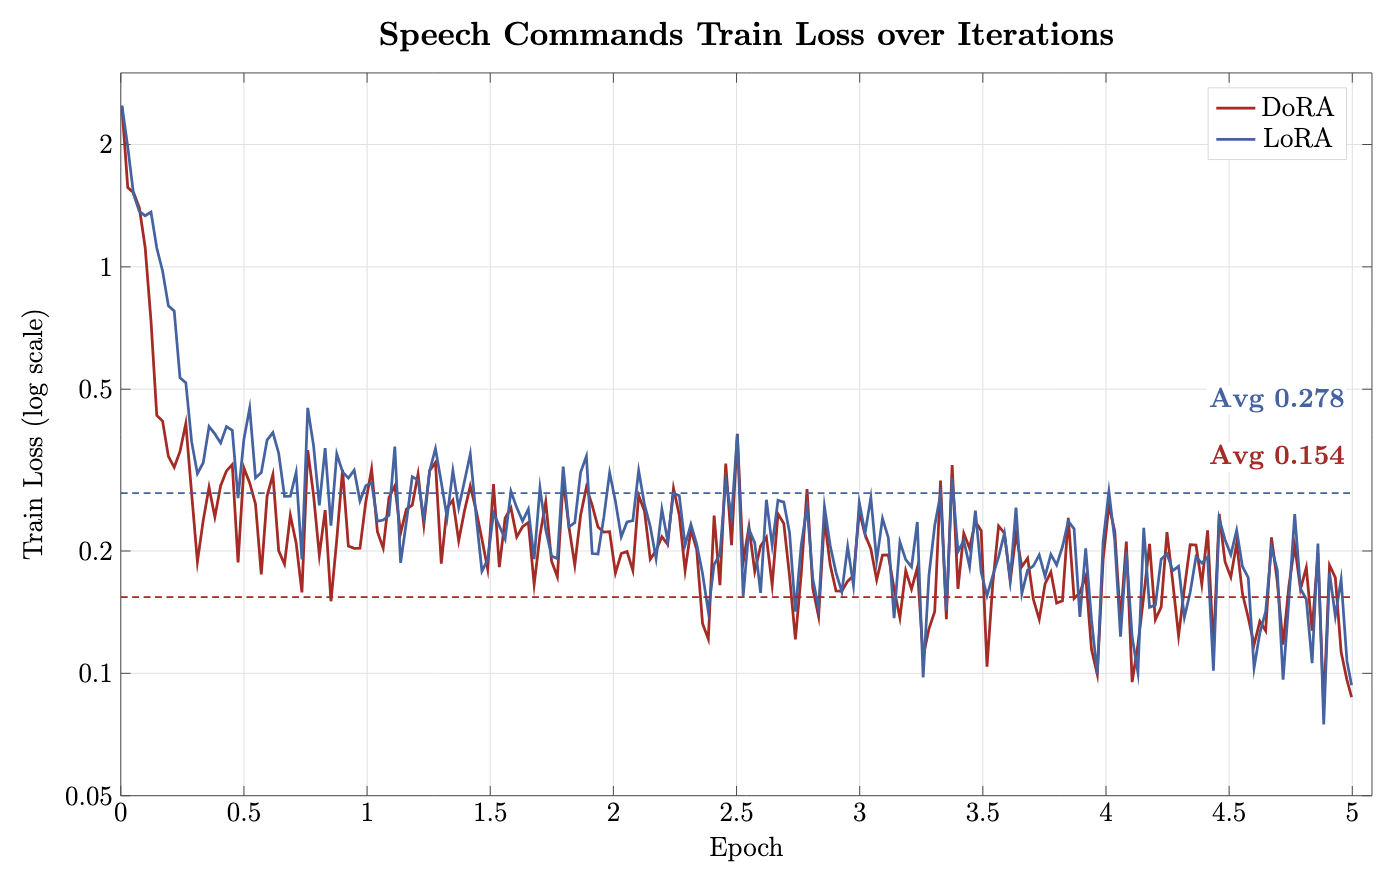
\includegraphics[width=0.54\linewidth,height=40.0cm,keepaspectratio]{wav2vec2loss2.png}

				\end{center}
				{\small\textit{\hl{-44.6\% average train loss.} DoRA shows lower average training loss, suggesting faster optimization and smoother convergence.}}
			\end{tcolorbox}

		\end{column}

		% ============================================================
		%  COLUMN 2  —  NLP + Audio Results  (unchanged)
		% ============================================================
		\begin{column}{0.37\textwidth}

			\begin{tcolorbox}[posterblock,title=NLP Results]
				\lb{Cross-Task at $r=8$} (RoBERTa-base accuracy / F1+acc / accuracy)

				\vspace{0.2cm}
				\begin{center}\small
					\begin{tabular}{@{}lcccc@{}}
						\toprule
						\textbf{Task}           & \textbf{DoRA}                     & \textbf{LoRA} & \textbf{FFT} & $\Delta$    \\
						\midrule
						SST-2 (67k, sentiment)  & 93.2\%                            & 93.3\%        & 93.2\%       & $-0.1$      \\
						MRPC (3.7k, paraphrase) & 87.8\%                            & 85.9\%        & 74.8\%       & $+1.9$      \\
						\rowcolor{TableShade}
						RTE (2.5k, inference)   & \textbf{70.0\%}                   & 66.1\%        & 54.9\%       & $\bm{+3.9}$ \\
						\midrule
						SST-2 \textit{large}    & 96.4\%                            & 95.5\%        & 95.4\%       & $+0.9$      \\
						MRPC \textit{large}     & 89.3\%                            & 89.5\%        & 80.6\%       & $-0.2$      \\
						RTE  \textit{large}     & 76.9\%                            & 78.7\%        & 68.6\%       & $-1.8$      \\
						\midrule
						% TinyLlama-1.1B          & \textbf{96.0\%} & ---           & ---          & ---         \\
						OpenLLaMA-3B            & 81.0\%\textsuperscript{$\dagger$} & ---           & ---          & ---         \\
						\bottomrule
					\end{tabular}
				\end{center}

				\vspace{0.15cm}
				\small\textit{DoRA's advantage is largest on \hl{low-data tasks}
					(RTE $+3.9$\,pp) where magnitude decoupling reduces directional
					gradient interference.  On large models both methods saturate.}

				\vspace{0.40cm}
				\lb{Benchmark Task Examples} (Text $\rightarrow$ Label)

				\vspace{0.30cm}
				{\footnotesize
					\begin{tabularx}{\linewidth}{@{} l X r @{}}
						\textbf{SST-2}
						 & ``\textit{...crowd-pleasing as a documentary can get.}''
						 & $\to$ \hl{Positive}                                                                                    \\[2pt]
						\textbf{MRPC}
						 & S1: ``\textit{Corixa rose 54c to \$7.74.}''\ \ S2: ``\textit{...rose 54c, or 8\%, to \$7.74.}''
						 & $\to$ \hl{Not Equiv.}                                                                                  \\[2pt]
						\textbf{RTE}
						 & P: ``\textit{Leaders signed Egypt--Israel treaty in 1979.}''\ \ H: ``\textit{Treaty signed in 1979.}''
						 & $\to$ \hl{Not Entailed}                                                                                \\
					\end{tabularx}}

				\vspace{0.25cm}

				\begin{center}
					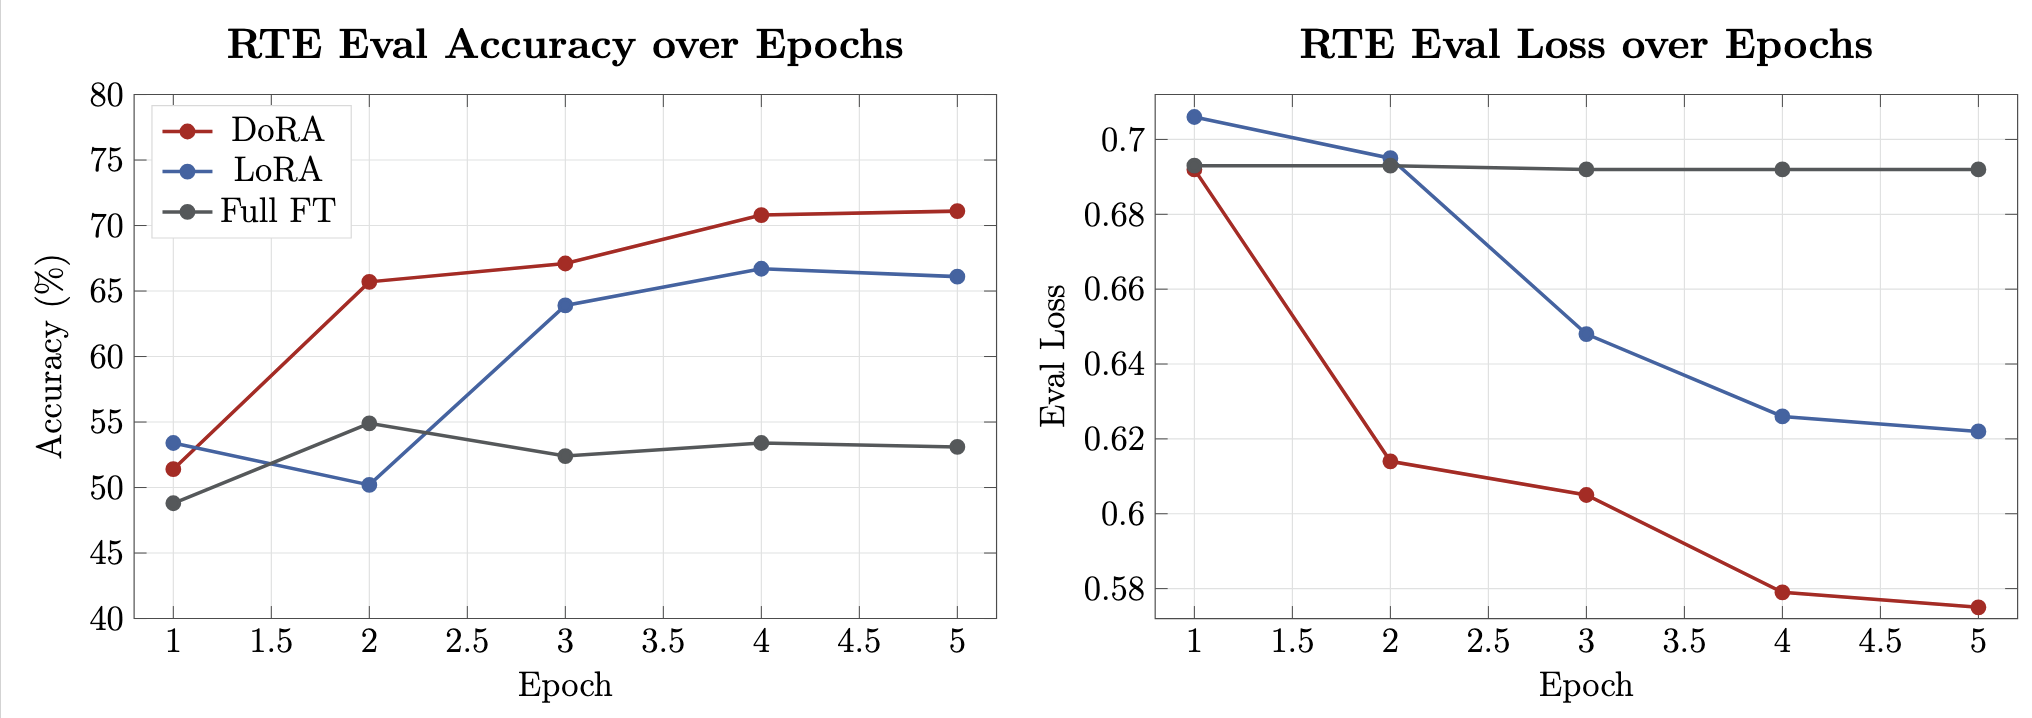
\includegraphics[width=1\linewidth]{rte_learning_curves.png}
					\small\textit{DoRA converges faster and to a lower eval loss than LoRA on RTE, while full fine-tuning stalls near the random-guess baseline.}

				\end{center}

				\lb{Magnitude-Direction Updates} (Full vs. LoRA vs. DoRA)

				\vspace{0.4cm}
				\begin{center}
					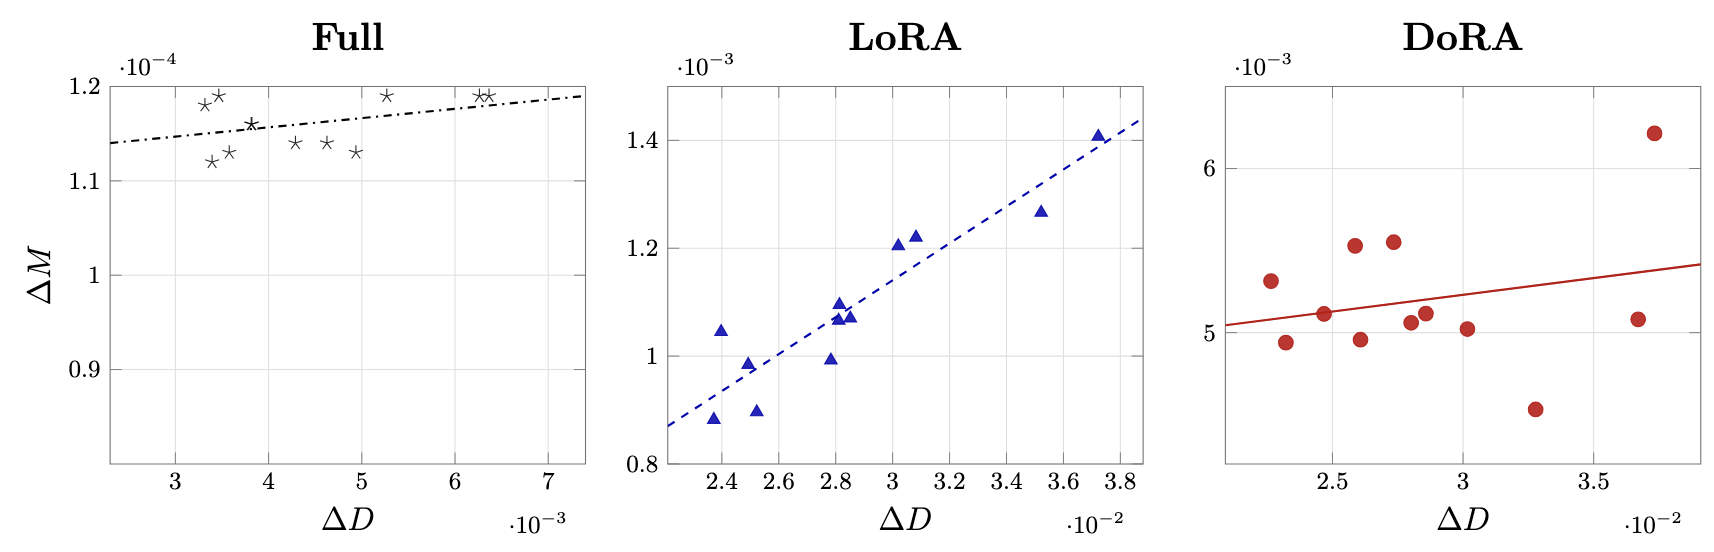
\includegraphics[width=0.9\linewidth]{magnitude-direction.png}
				\end{center}

				\vspace{0.15cm}
				\small\textit{\hl{Full r = 0.40, LoRA r = 0.93, DoRA r = 0.24}. DoRA shows significantly lower slope and correlation than LoRA, closer to FFT, showing the effect of de-coupling $\bold{M}$ and $\bold{D}$.}

			\end{tcolorbox}


		\end{column}

		% ============================================================
		%  COLUMN 3  —  Vision/VLA Samples + Conclusions  (unchanged)
		% ============================================================
		\begin{column}{0.29\textwidth}

			\begin{tcolorbox}[posterblock,title=Vision \& Robot Results]
				\lb{Object Grasping} Predict a 2-D bounding box around the
				graspable object in an RGB tabletop image. Frozen ViT-B/16
				and SigLIP-B/16 backbones, adapted at $r{=}8$, scored by IoU.

				\vspace{0.2cm}
				\begin{center}\small
					\begin{tabular}{@{}lcc@{}}
						\toprule
						\textbf{Backbone} & \textbf{DoRA}       & \textbf{LoRA} \\
						\midrule
						ViT-B/16          & 11.9\% IoU          & 11.9\% IoU    \\
						\rowcolor{TableShade}
						SigLIP-B/16       & \textbf{22.0\%} IoU & 21.5\% IoU    \\
						\bottomrule
					\end{tabular}
				\end{center}

				\vspace{0.15cm}
				\small\textit{SigLIP's richer vision--language pretraining benefits
					more from magnitude decoupling. ViT features show minimal difference.}

				\vspace{0.25cm}
				\lb{Qualitative: SigLIP + DoRA}
				{\small Green = predicted grasp\quad Red = ground truth}

				\vspace{0.15cm}
				\begin{center}
					\begin{tabular}{@{}ccc@{}}
						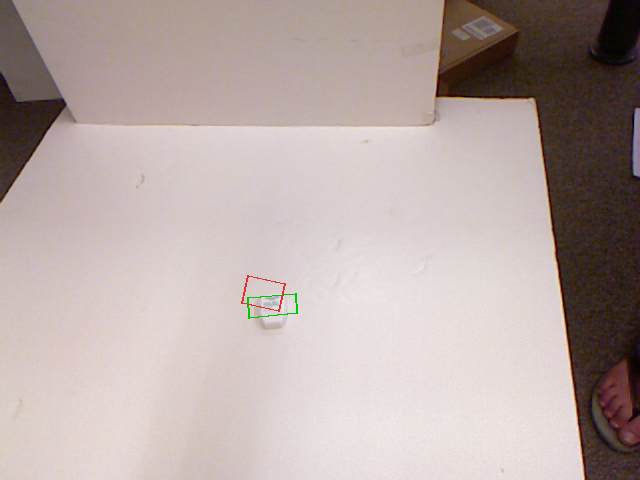
\includegraphics[width=6.3cm,height=5.2cm,
							clip]{grasp_siglip_09.png} &
						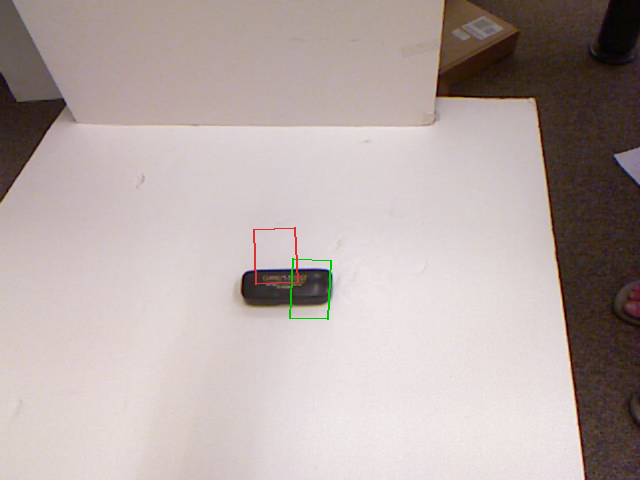
\includegraphics[width=6.3cm,height=5.2cm,
							clip]{grasp_siglip_04.png} &
						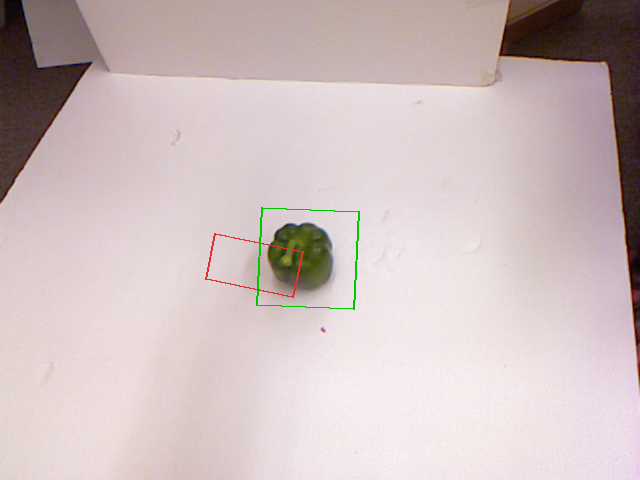
\includegraphics[width=6.3cm,height=5.2cm,
							clip]{grasp_siglip_00.png}
					\end{tabular}
				\end{center}

				\vspace{0.25cm}
				\lb{Push-T VLA Task}
				A robot slides a T-shaped block to a target pose from an
				overhead camera plus language instruction. DoRA adapts a
				126-layer OpenVLA model; action MSE drops 63.6 $\to$
				\textbf{27.9} over 3 epochs.

				\vspace{0.15cm}
				\begin{center}
					\begin{tabular}{@{}cc@{}}
						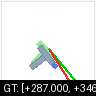
\includegraphics[width=7.0cm,height=4.8cm,
							clip]{pusht_00.png} &
						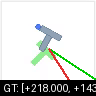
\includegraphics[width=7.0cm,height=4.8cm,
							clip]{pusht_04.png}
					\end{tabular}
				\end{center}
				\vspace{0.1cm}
				\centering{\small\textit{DoRA adapter driving Push-T rollouts}}
			\end{tcolorbox}

			\begin{tcolorbox}[posterblock,title=Conclusions]
				{\small\begin{itemize}\setlength{\itemsep}{0.04cm}\setlength{\topsep}{0pt}
						\item \hl{Low-data NLP:} DoRA gains most when data is scarce —
						      RTE $+3.9$\,pp, MRPC $+3.0$\,pp at $r{=}16$.
						\item \hl{Audio:} $+0.7\%$ test acc.\ and 25\% faster training on
						      Wav2Vec2 — directional convergence is faster.
						\item \hl{Vision:} SigLIP amplifies DoRA's benefit ($+0.5$\,pp IoU);
						      ViT-base does not, meaning base models matter.
					\end{itemize}}
			\end{tcolorbox}

			\begin{tcolorbox}[posterblock,title=Future Work]
				{\small\begin{itemize}\setlength{\itemsep}{0.03cm}\setlength{\topsep}{0pt}
						\item \hl{QLoRA + DoRA:} 4-bit quantized fine-tuning to reach 7B+ models on consumer hardware.
						\item \hl{Diffusion models:} apply DoRA to action-distribution heads and image-generation U-Nets.
						\item \hl{SVD-based decomposition:} explore EDoRA [7] — uses SVD to decouple singular directions, potentially reducing the parameter budget beyond DoRA.
					\end{itemize}}
			\end{tcolorbox}


		\end{column}

	\end{columns}

\end{frame}
\end{document}